\documentclass[UTF8]{ctexart}
\usepackage{hyperref}
\usepackage{abstract}
\usepackage[margin=1in]{geometry}
\usepackage{graphicx}
\begin{document}

\title{弹簧振子实验}
\author{2019012137  物理92  张鸿琳}
\maketitle
\begin{abstract}
本实验目的是探究弹簧的一些性质,包括其劲度系数和振动特性,实验有两个主要部分:①由胡克定律测定弹簧的劲度系数 ②研究弹簧振子的振动特性,验证周期公式。在测量劲度系数的实验中,不断改变砝码质量,测量其对应的弹簧形变量,再根据胡克定律 F=kx,利用最小二乘法,拟合出k的大小;在验证弹簧振动周期的实验中,也不断改变砝码质量,将其偏离平衡位置一定距离,记录其50个周期的时间,再次利用最小二乘法,拟合出曲线,验证了公式$T=2\pi\sqrt{\frac{m}{k}}$的正确性,通过对比前后两个实验得到的劲度系数,更进一步确定了整个实验的合理性和正确性。



\centering
\textbf{Keywords:}弹簧性质,劲度系数,周期公式,最小二乘法
\end{abstract}

\newpage
\tableofcontents
\newpage
\section{数据处理}
\subsection{由胡克定律测定弹簧的劲度系数}
(本实验原始数据见“原始测量数据”表一)
\newline
在已知重力加速度为9.8$m/s^2$的条件下,由胡克定律F=kx,可得二者应符合线性相关的关系,设砝码质量为$m_i$,则测得的拉力$F_i$=$m_i$g,其对应的弹簧形变量为$\Delta l_i$,则二者应大致符合方程F=$b_1$$\Delta l$,故利用实验数据,得$\bar{F}$=1.715 N,$\bar{\Delta l}$=0.3561667 m,使用最小二乘法公式:

$$b_1=\frac{\sum(\Delta l_i-\bar{\Delta l})F_i}{\sum(\Delta l_i-\bar{\Delta l})^2}$$,$$b_0=\bar{F}-b_1\bar{\Delta l}$$
得到$b_1$=4.849808283(单位均换算至国际单位制),拟合图像如下图:
\begin{center} 
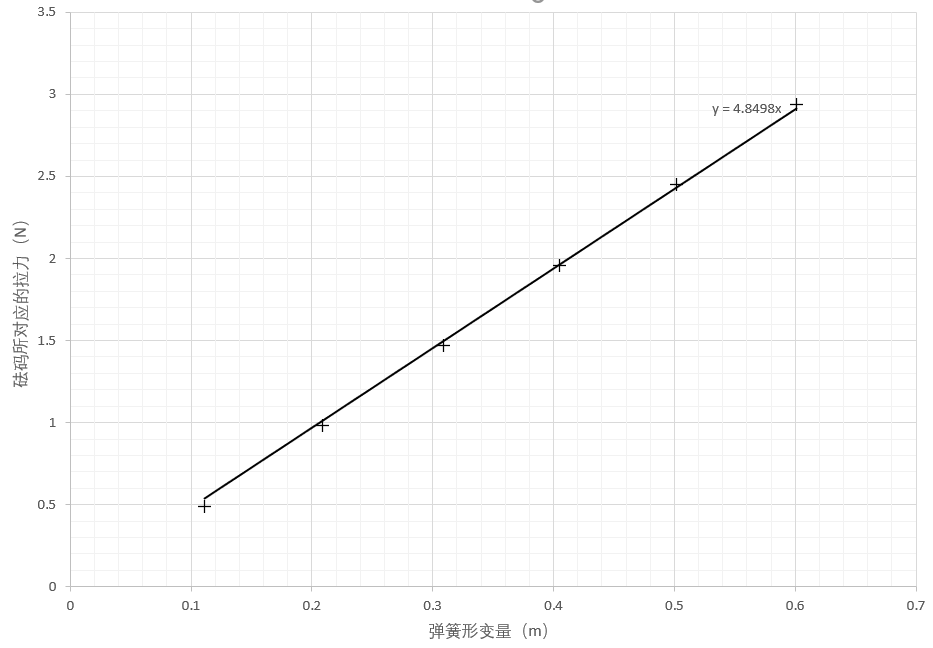
\includegraphics[width=0.95\textwidth]{BB.png} 
\end{center}

标准偏差$s_k=\sqrt{\frac{\sum [F_i-(b_0+b_1\Delta l_i)]^2}{(n-1)\sum(\Delta l_i-\bar\Delta l)^2}}$=0.078591242,
劲度系数不确定度$U_k=t_{(v=n-1)} s_k$=$2.570582\times 0.078591242$=0.202025218,
劲度系数相对不确定度$\frac{U_k}{k}$=0.041656331,
故而劲度系数k=$b_1=(4.85\pm 0.20) N/m$,
弹簧形变量相对不确定度为$\frac{U_{\Delta l}}{\bar \Delta l}\approx$$10^{-1}$
\newline
(数据比较部分见“讨论”)

\subsection{研究弹簧振子的振动特性,验证周期公式}
(本实验原始数据见“原始测量数据”表二)
\newline
由弹簧振子的振动周期公式$T=2\pi\sqrt{\frac{m}{k}}$,变换得$m_i=k(\frac{T_i}{2\pi})^2$,可见如果把$m_i$和$\frac{T_i}{2\pi}$当做两个变量,二者线性相关,对原始数据稍作处理,得到下表:
\begin{table}[htbp!] 
\centering 
\begin{tabular}{|l|c|r|} 
\hline 
 砝码质量$m_i$(g) &  $(\frac{T_i}{2\pi})^2$   ($s^2$) \\ 
\hline 
 50 & 0.010015 \\ 
\hline 
 100 & 0.020028 \\ 
\hline 
 150 &  0.030161 \\ 
\hline 
 200 & 0.040036  \\ 
\hline 
 250 & 0.049832 \\ 
\hline 
 300 & 0.059980  \\ 
\hline
\end{tabular} 
\end{table}

同样利用最小二乘法,得到$b_1$=5.001415736拟合程度见下图:
\begin{center} 
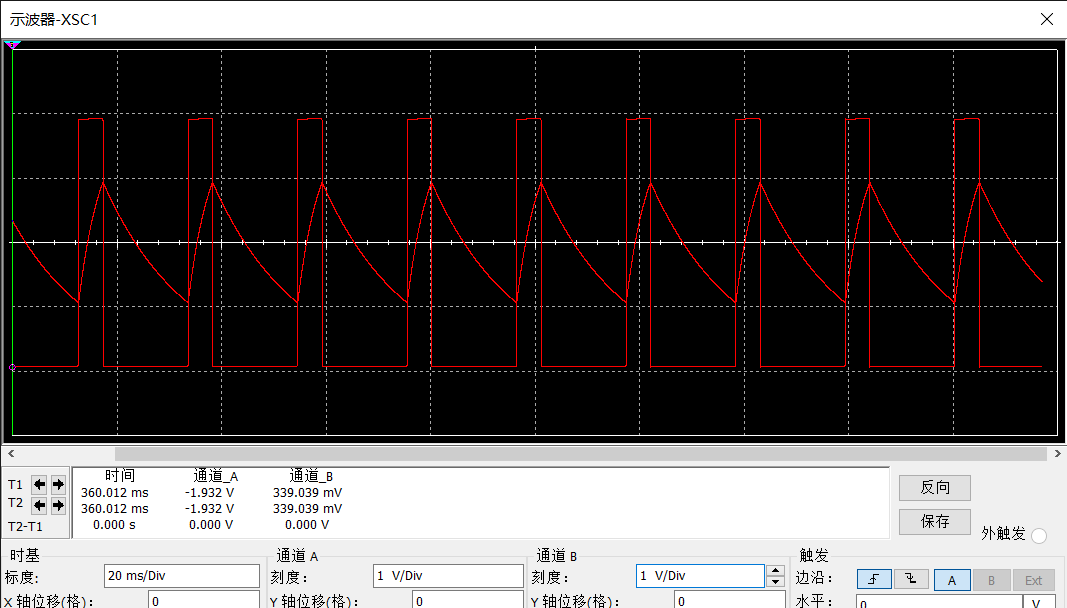
\includegraphics[width=0.95\textwidth]{CC.png} 
\end{center}
标准偏差$s_k=\sqrt{\frac{\sum [m_i-(b_1(\frac{T_i}{2\pi})^2)]^2}{(n-1)\sum((\frac{T_i}{2\pi})^2-\bar(\frac{T_i}{2\pi})^2)^2}}$=0.012706317,
不确定度为$U_k=t_{(v=n-1)} s_k$=0.032662627,
相对不确定度为$\frac{U_k}{k}$=0.006530676,
故而劲度系数k=($5.001\pm 0.033$) N/m,
估计周期测量的相对不确定度数量级$U_T\approx$$10^{-2}$(根据资料人反应延迟约为0.2秒)
\newline
(数据比较部分见“讨论”)

\section{讨论}
\subsection{一些数据的比较}
首先在第一组实验中,劲度系数和估计弹簧形变量相对不确定度相差一个数量级,所以可见弹簧形变量测量时产生的误差对于最终结果的影响较小;而相比之下,在第二组数据中,劲度系数和周期测量相对不确定度数量级相仿,所以在周期判定上的误差对于最终结果影响较大。该现象的发生可以从二者的方程中看出,$\Delta l$位于一次项中,而T位于二次项中,所以很明显,T容易产生更大的对结果的影响。


另外,再比较两个实验的最终结果,有一定差距,但是在各自不确定度范围内二者有交叉部分,位于4.9 N/m左右,证明整个实验是基本正确,合理的,而且,第一个实验的不确定度明显大于第二个实验,说明第一个实验,虽然单位弹簧形变量误差相较于单位周期判定误差往往产生较小的影响,但是由于形变量误差本身就较大,所以最终产生了相较于第二个实验中周期判定误差产生的影响更大的影响,所以相比之下,第二个实验的结果更具有说服力和可信度,有理由相信,劲度系数更接近于5 N/m。
\subsection{对于实验数据比较的思考和对实验本身的反思}
由上述两个比较来看,在一般日常实验中,由于人对周期的判定更为灵敏,所以更适宜采用第二种方法来测定某一弹簧的劲度系数,但是如果有更为灵敏的测量仪器,则要考虑到从本质来讲,第一个实验中对长度测量引起的误差往往更容易产生较小的影响。


就实验本身来讲,两个实验不确定度其实都较高,精度较高的第二个实验不确定度仍然达到了6\%左右,当然很大程度上是实验者本身测量行为产生的影响,但也一定程度说明了实验本身确实存在可改进的地方,比如在第一个实验中使用更加精密的测量仪器,在第二个实验中,采取机器判定、计时的方法等可以明显增加精度。
\section{原始测量数据}
\subsection{“由胡克定律测定弹簧的劲度系数”的原始数据}
在第一个实验中,由网站模拟出了下列数据:
\begin{table}[htbp!] 
\centering 
\begin{tabular}{|l|c|r|} 
\hline 
 砝码质量$m_i$(g) &  弹簧形变量$\Delta l_i$(cm)  \\ 
\hline 
 50 & 11.1  \\ 
\hline 
 100 & 20.9 \\ 
\hline 
 150 & 30.9  \\ 
\hline 
 200 & 40.5  \\ 
\hline 
 250 & 50.2  \\ 
\hline 
 300 & 60.1  \\ 
\hline
\end{tabular} 
\end{table}
\subsection{“研究弹簧振子的振动特性,验证周期公式”的原始数据}
在第二个实验中,由网站模拟出了下列数据:
\begin{table}[htbp!] 
\centering 
\begin{tabular}{|l|c|r|} 
\hline 
 砝码质量$m_i$(g) &  50个振动周期耗时$T_{50}$(s)  \\ 
\hline 
 50 & 31.44 \\ 
\hline 
 100 & 44.46 \\ 
\hline 
 150 & 54.56  \\ 
\hline 
 200 & 62.86  \\ 
\hline 
 250 & 70.13 \\ 
\hline 
 300 & 76.94  \\ 
\hline
\end{tabular} 
\end{table}
\begin{thebibliography}{123456} 
\bibitem{ref1} 朱鹤年. 新概念基础物理实验讲义. 清华大学出版社. 2013. 
\bibitem{ref2} PhET:免费的在线物理、化学、生物、地理及数学仿真程序
\bibitem{ref3} Carl Wieman Biographical
\bibitem{ref4} Carl Edwin Wieman, Magnet Academy from the National High Magnetic Field Laboratory 
\end{thebibliography}


\end{document}
